\chapter{Experimental Results and Analysis}
\label{sec:experimental-results}

\section{Results Analysis}
This chapter presents the results obtained from the three experiments. The findings are reported separately for filesystem-level inspection, TRIM-enabled and TRIM-disabled recovery conditions, storage-device type, filesystem utilisation, recovery delay, and TRIM execution time.
The results are interpreted using the distinction between logical deletion, host-side recoverability, and physical sanitization. A file may disappear from the filesystem while data remains in storage areas that cannot be observed through ordinary host-level access. Similarly, an absence of recovered signatures indicates that the selected recovery procedure did not identify the data, but it does not independently prove that all physical copies have been erased.

\subsection{Experiment 1: TRIM and Filesystem-Level Data Recoverability}

\subsubsection{Inode State After Deletion and TRIM}
The inode examination showed that the deleted file had been logically removed from the ext4 filesystem. The inode reported a size of zero and a block count of zero. Its link count was also zero, indicating that no directory entry referenced the inode. The extent tree was empty, showing that no usable block pointers remained in the inode.
The debugfs stat command returned the following inode information after deletion:

\begin{verbatim}
Inode: 6291458   Type: regular    Mode:  0644   Flags: 0x80000
Generation: 2405750640    Version: 0x00000000:0000005c
User:     0   Group:     0   Project:     0   Size: 0
File ACL: 0
Links: 0   Blockcount: 0
Fragment:  Address: 0    Number: 0    Size: 0
 ctime: 0x6a86c9f3:ad975988 -- Thu Aug 20 11:33:39 2026
 atime: 0x6a86c7cc:115e960c -- Thu Aug 20 11:24:28 2026
 mtime: 0x6a86c9f3:ad975988 -- Thu Aug 20 11:33:39 2026
 crtime: 0x6a86c7cc:115e960c -- Thu Aug 20 11:24:28 2026
 dtime: 0x6a86c9f3:(ad975988) -- Thu Aug 20 11:33:39 2026
Size of extra inode fields: 32
Inode checksum: 0xbe4252c1
EXTENTS:
\end{verbatim}

Several observations from the inode state are significant:

\begin{itemize}
    \item \textbf{Size and Blockcount:} Both were zero, indicating that the file content had been logically unlinked from the inode. The Size: 0 and Blockcount: 0 
    fields confirm that the inode no longer references any data blocks.

    \item \textbf{Links:} The Links: 0 value indicates that no directory entries reference this inode, confirming it was unlinked.

    \item \textbf{Deletion Timestamp:} The dtime field was set to the deletion time (Thu Aug 20 11:33:39 2026), confirming that the inode had been deallocated.

    \item \textbf{EXTENTS:} The extent tree was empty, meaning no block pointers were retained in the inode.

    \item \textbf{Inode Type and Flags:} The inode remained marked as type regular with flags 0x80000, but the loss of block pointers made data recovery through 
    filesystem metadata impossible.
\end{itemize}
The deletion timestamp was recorded in the inode. This timestamp provides forensic evidence that the inode had been deallocated, but it does not provide a mechanism for recovering the file content. The inode remained identifiable as a regular file, but its filesystem references to data blocks had been removed. These observations demonstrate successful logical deletion at the filesystem level. They do not, by themselves, establish whether copies of the file remained in physical NAND pages, remapped blocks, over-provisioned regions, or controller-managed areas.
\subsubsection*{Journal State Comparison}

The journal state before and after deletion showed an important distinction. The journal checksum changed after deletion while the journal sequence number remained unchanged. This indicates that deletion-related metadata had been written to the journal. The journal therefore preserved evidence of filesystem activity associated with deletion.

Before deletion:

\begin{verbatim}
Journal sequence: 0x0000003d
Journal checksum: 0x0cd525e3
\end{verbatim}

After deletion:

\begin{verbatim}
Journal sequence: 0x0000003d
Journal checksum: 0x92f1d2b1
\end{verbatim}


\subsubsection*{ext4magic Recovery Attempt}

The ext4magic recovery produced the following output:

\begin{verbatim}
Filesystem in use: /dev/sda1

Dump internal Inode 6291458
Status : Inode is Unallocated

Inode: 6291458   Type: regular    Mode:  0644   Flags: 0x80000
...
ext4magic : EXIT_SUCCESS
\end{verbatim}

The tool reported that the inode was unallocated (Status : Inode is Unallocated) and could not recover the file content. Even when the journal start block was specified, 
ext4magic was unable to reconstruct the file. The output "Dump Filesystemblock 620 Status : Block is Allocated" indicated that the journal block itself was present but 
contained no recoverable file data.

\subsubsection*{Pathname Resolution}

The ncheck command returned no pathname for the inode:

\begin{verbatim}
debugfs: ncheck 6291458
Inode	Pathname
debugfs: q
\end{verbatim}

This confirmed that no directory entry pointed to the inode, consistent with the file having been unlinked.

\subsubsection*{Inode Map Location}

The imap command identified the inode's location in the filesystem:

\begin{verbatim}
Inode 6291458 is part of block group 768
    located at block 25165856, offset 0x0100
\end{verbatim}

This information confirmed that the inode was physically present but its contents had been cleared.

\subsubsection*{Journal Log Analysis}

The journal logdump revealed the transactions that had been written during the deletion process:

\begin{verbatim}
Journal starts at block 620, transaction 61
Found expected sequence 61, type 1 (descriptor block) at block 620
Found expected sequence 61, type 2 (commit block) at block 626
Found expected sequence 62, type 1 (descriptor block) at block 627
Found expected sequence 62, type 2 (commit block) at block 633
Found expected sequence 63, type 1 (descriptor block) at block 634
Found expected sequence 63, type 2 (commit block) at block 637
Found expected sequence 64, type 5 (revoke table) at block 638
Found expected sequence 64, type 1 (descriptor block) at block 639
Found expected sequence 64, type 2 (commit block) at block 652
No magic number at block 653: end of journal.
\end{verbatim}

The journal contained four transactions (61–64) related to the deletion. Notably, transaction 64 included a revoke table (type 5), which is used to indicate that 
certain blocks should no longer be considered valid in the journal. This revocation mechanism is relevant to filesystem-level recoverability after deletion.

The detailed descriptor block dump showed which filesystem blocks were logged:

\begin{verbatim}
Dumping descriptor block, sequence 64, at block 639:
  FS block 25174048 logged at journal block 640 (flags 0x0)
  FS block 25165856 logged at journal block 641 (flags 0x2)
  FS block 9504 logged at journal block 642 (flags 0x2)
  FS block 25165825 logged at journal block 643 (flags 0x2)
  FS block 13 logged at journal block 644 (flags 0x2)
  FS block 2097166 logged at journal block 645 (flags 0x2)
  FS block 2 logged at journal block 646 (flags 0x2)
  FS block 25165840 logged at journal block 647 (flags 0x2)
  FS block 26214432 logged at journal block 648 (flags 0x2)
  FS block 30933001 logged at journal block 649 (flags 0x2)
  FS block 15 logged at journal block 650 (flags 0x2)
  FS block 26214416 logged at journal block 651 (flags 0xa)
\end{verbatim}

The journal blocks included inodes and metadata blocks but did not contain the actual file data blocks, which explains why ext4magic could not recover the file content.

\subsubsection*{Direct Block Inspection}

The direct inspection of previously allocated data blocks showed that they contained zero bytes:

\begin{verbatim}
sudo dd if=/dev/sda1 bs=4096 skip=33388 count=1 2>/dev/null| xxd| head -20
00000000: 0000 0000 0000 0000 0000 0000 0000 0000  ................
00000010: 0000 0000 0000 0000 0000 0000 0000 0000  ................
...
\end{verbatim}

Both previously allocated blocks (33388 and 33389) contained only zeros. This indicates that the data blocks had been sanitized—either through the TRIM operation itself, 
through subsequent garbage collection, or through the filesystem's block deallocation process that returned them to the free list.

\subsubsection*{Journal Inode Extraction}

The extracted inode portions from the journal blocks confirmed that no recoverable inode data remained:

\begin{verbatim}
sudo dd if=~/inode_analysis/journal_tx61.bin 
of=~/inode_analysis/inode_tx61.bin bs=1 skip=256 count=256
\end{verbatim}

The extracted journal inode showed that the journal recorded the inode in its deallocated state, with zero size and block count, consistent with the debugfs stat output.

The experimental results demonstrate several important characteristics of filesystem-level recoverability after deletion and TRIM. The inode state after deletion shows 
that ext4 fully deallocates the inode when a file is removed. The inode's block pointers are cleared (Blockcount: 0, empty EXTENTS), the size is set to zero (Size: 0), 
and the link count is set to zero (Links: 0). The dtime field records the deletion time, which is a forensic indicator but does not assist in data recovery. This 
deallocation pattern is consistent with the standard ext4 deletion behavior described in the filesystem documentation: when a file is unlinked, the inode is marked as 
free and its block pointers are cleared to prevent the filesystem from treating stale block references as valid. The journal analysis reveals that the deletion was 
recorded in the journal, but the journal contained only metadata updates, not the actual file data. This is expected behavior for the ext4 filesystem in its default 
data-ordered mode: metadata is journaled before it is written to the filesystem, but data blocks are not necessarily journaled. Consequently, while the journal can be 
used to recover filesystem metadata after a crash, it does not provide a reliable mechanism for recovering deleted file data. The revoke table in transaction 64 is 
particularly significant: it indicates that the journal explicitly invalidated certain blocks, further reducing the likelihood of recovery through journal replay. The 
direct block inspection showed that the previously allocated data blocks contained zero bytes. This is consistent with the TRIM operation having informed the SSD that 
the logical blocks were no longer in use, allowing the controller to discard the physical data. The zeros observed in the block inspection could reflect either physical 
erasure of the NAND cells or the controller returning zeroed data at the logical block level. Either interpretation is consistent with the conclusion that the data was 
not recoverable through host-side block access. 

\subsection{Experiment 2: Data Recovery After TRIM}
Experiment 2 evaluated whether deleted data could be recovered from the NVMe and SATA SSDs under nominal TRIM-enabled and TRIM-disabled conditions. Recovery was 
assessed by counting dataset-specific signatures identified in the PhotoRec output. Each dataset contained 5,052 expected signatures, and five repeated runs were 
conducted for each storage configuration. The results are presented separately for the NVMe and SATA SSDs because the two devices produced different recovery patterns

\subsection*{NVMe SSD Results}
\begin{table}[H]
    \centering
    \caption{Data Recovery Results After TRIM on NVMe SSD}
    \label{tab:nvme-recovery-results}

        \begin{tabular}{c c c c c c}
        \toprule
        \textbf{Dataset} &
        \multicolumn{5}{c}{\textbf{Signatures Recovered}} \\
        \cmidrule(lr){2-6}
        & \textbf{Run 1} & \textbf{Run 2} & \textbf{Run 3}
        & \textbf{Run 4} & \textbf{Run 5} \\
        \midrule
        DS1  & 5,052 & 5,052 & 5,052 & 5,052 & 5,052 \\
        DS2  & 0     & 0     & 0     & 0     & 0     \\
        DS3  & 5,052 & 5,052 & 5,052 & 5,052 & 5,052 \\
        DS4  & 0     & 0     & 0     & 0     & 0     \\
        DS5  & 5,052 & 5,052 & 5,052 & 5,052 & 5,052 \\
        DS6  & 5,052 & 5,052 & 5,052 & 5,052 & 5,052 \\
        DS7  & 5,052 & 5,052 & 5,052 & 5,052 & 5,052 \\
        DS8  & 5,052 & 5,052 & 5,052 & 5,052 & 5,052 \\
        DS9  & 5,052 & 5,052 & 5,052 & 5,052 & 5,052 \\
        DS10 & 5,052 & 5,052 & 5,001 & 5,001 & 0 \\
        DS11 & 5,052 & 5,052 & 5,052 & 5,052 & 5,052 \\
        DS12 & 5,052 & 5,052 & 5,052 & 0     & 0 \\
        DS13 & 5,052 & 5,052 & 5,052 & 5,052 & 5,052 \\
        DS14 & 5,052 & 5,052 & 5,052 & 5,052 & 5,052 \\
        DS15 & 5,052 & 5,052 & 5,052 & 5,052 & 5,052 \\
        DS16 & 5,052 & 5,052 & 5,052 & 5,052 & 5,052 \\
        \bottomrule
    \end{tabular}
\end{table}

\begin{figure}[H]
    \centering
    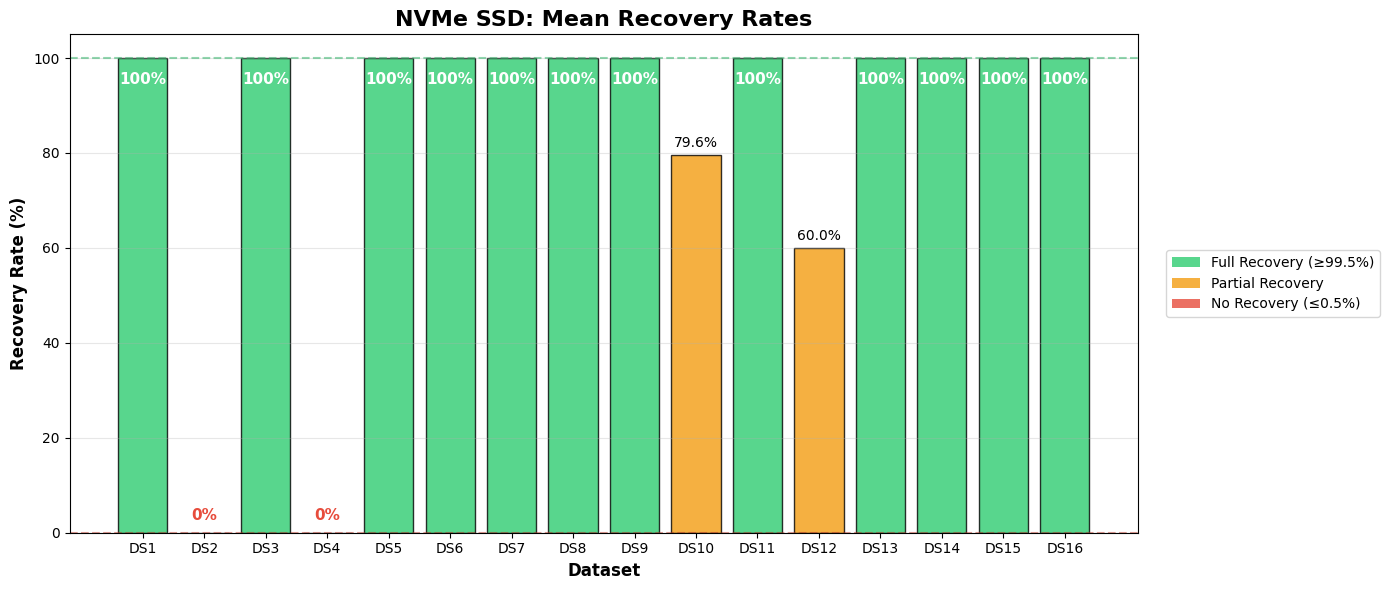
\includegraphics[width=0.8\textwidth]{images/nvme_mean_recov.png}
    \caption{Mean Recovery on NVMe SSD}
    \label{fig:nvme_recovery}
\end{figure}

The NVMe results showed that the recovery procedure was effective for datasets that remained available on the device. The kept datasets, DS1, DS3, DS5, DS9, DS11, and 
DS13, each produced 5,052 recovered signatures in all five runs. This represents a recovery rate of 100\% for every kept dataset. These results provide a positive 
control because they demonstrate that the recovery tool was able to scan the device and identify the embedded dataset signatures when the data had not been removed. 

The post-deletion write datasets, DS6 to DS8 and DS14 to DS16, also produced 5,052 recovered signatures in every run. Their recovery rates were therefore 100\%. The 
recovery of these datasets confirms that the later write stage produced data that could be identified by the recovery procedure. However, their recovery should not be 
interpreted as recovery of the earlier deleted datasets. Instead, these datasets functioned as a separate test of whether newly written data remained observable after 
the deletion stage. 

The results for the deleted datasets under the nominal TRIM-enabled condition were considerably different. DS2 and DS4 produced zero recovered signatures in every run. 
Consequently, both datasets recorded a mean recovery rate of 0\%. The consistency of this result across all five repetitions indicates that no dataset-specific 
signatures from DS2 or DS4 were identified after deletion and the subsequent TRIM operation.

The two deleted datasets under the nominal TRIM-disabled condition produced substantially higher recovery rates. DS10 produced 5,052 signatures in the first two runs, 
5,001 signatures in the third and fourth runs, and zero signatures in the fifth run. The mean number of recovered signatures was 4,021.2, corresponding to a mean 
recovery rate of 79.60\%. DS12 produced 5,052 signatures in each of the first three runs and zero signatures in the final two runs. Its mean number of recovered 
signatures was 3,031.2, corresponding to a mean recovery rate of 60.00\%. 

The difference between the nominal TRIM-enabled and nominal TRIM-disabled results is therefore substantial on the NVMe SSD. The two deleted datasets under the 
TRIM-enabled condition produced a combined mean recovery rate of 0\%, whereas the two deleted datasets under the TRIM-disabled condition produced a simple average 
recovery rate of 69.80\%. This indicates that deleted data remained substantially more recoverable when the explicit TRIM operation was not performed.

The NVMe results also show considerable variability in the TRIM-disabled condition. DS10 had a standard deviation of approximately 44.50 percentage points, while DS12 
had a standard deviation of approximately 54.77 percentage points. The high variation resulted from the contrast between near-complete recovery in some runs and no 
recovery in other runs. Therefore, although the nominal TRIM-disabled condition allowed substantial recovery, the outcome was not identical across repeated experiments. 
This variability is particularly visible in DS12. The dataset was recovered almost completely in the first three runs, but no signatures were recovered in the final 
two runs. This indicates that the presence of deleted data was not sufficient by itself to guarantee successful recovery. The recoverability of the data changed between 
runs, suggesting that the state of the SSD, the storage controller, or the connection path influenced the final result.


\subsection*{SATA SSD Results}
\begin{table}[H]
    \centering
    \caption{Data Recovery Results After TRIM on SATA SSD}
    \label{tab:sata-recovery-results}

    \begin{tabular}{c c c c c c}
        \toprule
        \textbf{Dataset} &
        \multicolumn{5}{c}{\textbf{Signatures Recovered}} \\
        \cmidrule(lr){2-6}
        & \textbf{Run 1} & \textbf{Run 2} & \textbf{Run 3}
        & \textbf{Run 4} & \textbf{Run 5} \\
        \midrule
        DS1  & 5,052 & 5,052 & 5,052 & 5,070 & 5,052 \\
        DS2  & 56    & 19    & 0     & 0     & 0     \\
        DS3  & 5,052 & 5,052 & 5,052 & 5,052 & 5,052 \\
        DS4  & 47    & 37    & 0     & 0     & 0     \\
        DS5  & 5,052 & 5,052 & 5,052 & 5,052 & 5,052 \\
        DS6  & 5,052 & 5,052 & 5,052 & 5,052 & 5,052 \\
        DS7  & 5,052 & 5,052 & 5,052 & 5,052 & 5,103 \\
        DS8  & 5,052 & 5,052 & 5,052 & 5,052 & 5,103 \\
        DS9  & 5,052 & 5,052 & 5,052 & 5,052 & 5,052 \\
        DS10 & 56    & 0     & 0     & 0     & 0     \\
        DS11 & 5,052 & 5,052 & 5,052 & 5,052 & 5,052 \\
        DS12 & 72    & 4,487 & 0     & 0     & 0     \\
        DS13 & 5,052 & 5,052 & 5,052 & 5,052 & 5,052 \\
        DS14 & 5,052 & 5,052 & 5,052 & 5,052 & 5,052 \\
        DS15 & 5,052 & 5,052 & 5,052 & 5,052 & 5,052 \\
        DS16 & 5,052 & 5,052 & 5,052 & 5,052 & 5,052 \\
        \bottomrule
    \end{tabular}
\end{table}

\begin{figure}[H]
    \centering
    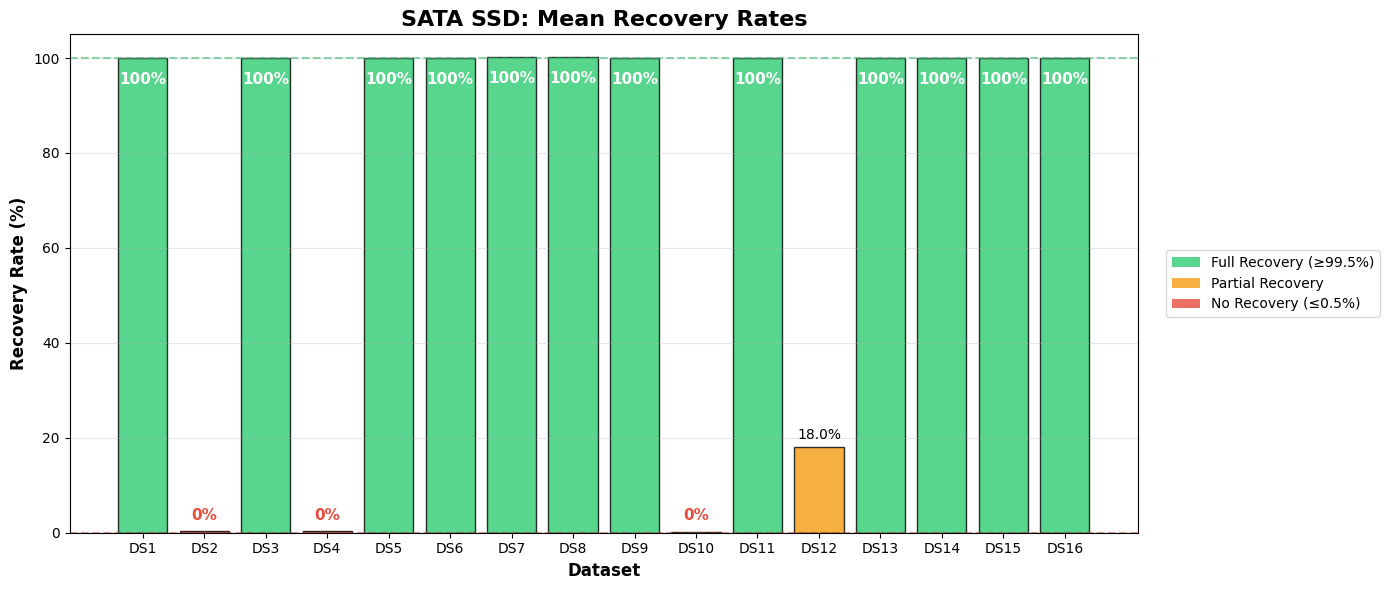
\includegraphics[width=0.8\textwidth]{images/sata_mean_recov.png}
    \caption{Mean Recovery on SATA SSD}
    \label{fig:sata_recovery}
\end{figure}

The SATA SSD results showed a similar pattern for the control datasets. DS3, DS5, DS9, DS11, and DS13 produced 5,052 signatures in all five runs. DS1 produced 5,052 
signatures in four runs and 5,070 signatures in one run. These results correspond to approximately 100\% recovery and confirm that the recovery procedure was capable of 
identifying the expected signatures on the SATA device. 

The post-deletion write datasets also showed almost complete recovery. DS6 produced 5,052 signatures in all five runs, while DS7 and DS8 produced 5,103 signatures in 
the fifth run and 5,052 signatures in the other four runs. DS14, DS15, and DS16 produced 5,052 signatures in every run. The mean recovery rates for these datasets were 
therefore approximately 100\%. The values slightly above 100\% resulted from the detection of more signature occurrences than the nominal expected value of 5,052 which 
were due to file remnants from previous runs being recovered by Photorec. 

The deleted datasets under the nominal TRIM-enabled condition produced only a small number of signatures in the first two runs and no signatures in the remaining three 
runs. DS2 produced 56, 19, 0, 0, and 0 signatures, resulting in a mean of 15 recovered signatures and a mean recovery rate of approximately 0.30\%. DS4 produced 47, 37, 
0, 0, and 0 signatures, resulting in a mean of 16.8 recovered signatures and a mean recovery rate of approximately 0.33\%. 

These results indicate that the nominal TRIM-enabled condition was highly effective at preventing recovery of the deleted signatures from the SATA SSD. However, the 
results should not be described as absolute zero recovery because small numbers of signatures were detected in the first two runs for both DS2 and DS4. A more accurate 
interpretation is that recovery was reduced to a near-zero level, with the remaining signatures appearing only during the initial repetitions.

The nominal TRIM-disabled SATA results were more variable than the TRIM-enabled results, but the overall recovery level remained substantially lower than that observed 
for the NVMe SSD. DS10 produced 56 signatures in the first run and zero signatures in the remaining four runs. This produced a mean recovery rate of only 0.22\%. DS12 
produced 72 signatures in the first run, 4,487 signatures in the second run, and zero signatures in the final three runs. Its mean recovery rate was 18.05\%. 

DS12 was the only SATA dataset to show a substantial recovery event under the nominal TRIM-disabled condition. The second run recovered 4,487 of the expected 5,052 
signatures, which corresponds to approximately 88.82\% recovery in that individual run. However, because no signatures were recovered in the final three runs, the mean
recovery rate across all five runs fell to 18.05\%. This demonstrates why the individual run results are important. Reporting only the mean would conceal the large 
difference between the second run and the other four runs.

The standard deviation for DS12 was approximately 39.57 percentage points, which reflects this inconsistent recovery pattern. By comparison, the standard deviation for 
DS10 was only approximately 0.50 percentage points because the dataset produced a small number of signatures in only the first run and zero signatures thereafter.


\subsection*{Comparison between the NVMe and SATA SSDs}
The comparison shows that the NVMe SSD retained considerably more recoverable data under the nominal TRIM-disabled condition than the SATA SSD. The NVMe deleted 
datasets produced mean recovery rates of 79.60\% and 60.00\%, whereas the corresponding SATA datasets produced mean recovery rates of 0.22\% and 18.05\%. Taking the 
simple average of the two deleted datasets, the nominal TRIM-disabled recovery rate was 69.80\% for the NVMe SSD and approximately 9.14\% for the SATA SSD.

Under the nominal TRIM-enabled condition, both devices produced very low recovery rates. The NVMe SSD produced no recovered signatures for either deleted dataset. The 
SATA SSD produced less than 1\% mean recovery for both deleted datasets. This indicates that the explicit TRIM operation was associated with a strong reduction in 
host-side recovery on both devices.

The results also demonstrate that TRIM behaviour was not uniform across the two SSDs. If the effect of TRIM were determined only by the operating-system deletion 
command, the two devices would be expected to show similar recovery patterns. Instead, the NVMe SSD showed substantial recovery when TRIM was disabled, while the SATA 
SSD showed limited recovery under the same nominal condition. This difference indicates that storage-device implementation and controller behaviour affected the 
persistence and recoverability of deleted data.

The results further show that repeated runs were necessary to identify the variability of the recovery process. The NVMe device produced large changes in recovery 
between runs for DS10 and DS12. The SATA device showed a similar pattern for DS12, where one run produced almost complete recovery while the other runs produced either 
minimal or no recovery. These results suggest that recovery should not be assessed using a single experimental run because a single run may either overestimate or 
underestimate the recoverability of deleted data.

\begin{figure}[H]
    \centering
    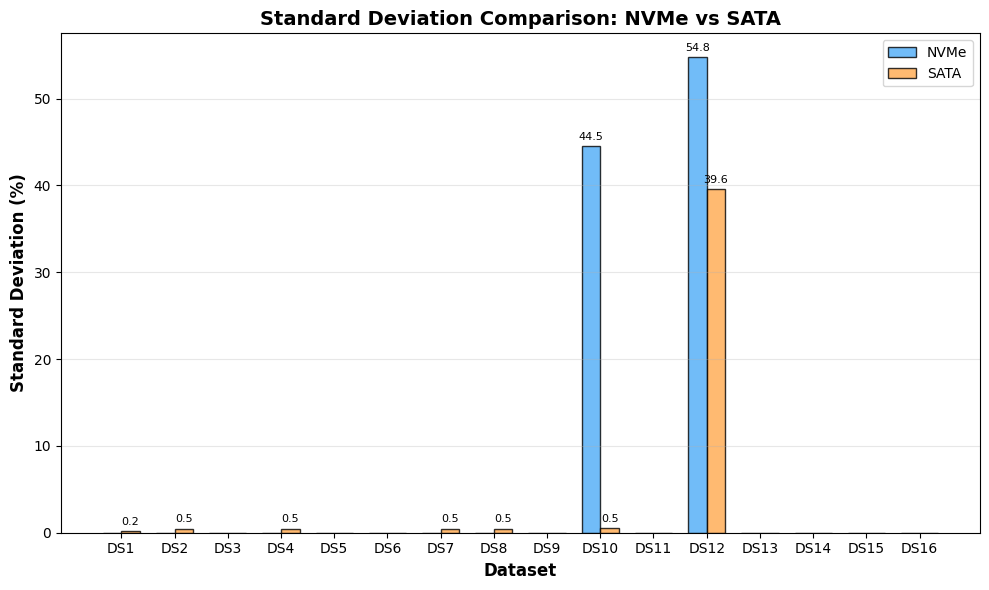
\includegraphics[width=0.8\textwidth]{images/sdv.png}
    \caption{Standard Deviation of Recovery on NVMe and SATA SSDs}
    \label{fig:sdv}
\end{figure}


The results provide evidence that the nominal TRIM-enabled condition substantially reduced the recovery of deleted dataset signatures on both storage devices. The 
reduction was complete for the NVMe deleted datasets and almost complete for the SATA deleted datasets. In contrast, disabling TRIM allowed substantial recovery on the 
NVMe SSD and limited, but occasionally significant, recovery on the SATA SSD.

The findings therefore support the conclusion that TRIM configuration influenced host-side data recoverability. However, the results do not support the broader 
conclusion that TRIM always produces the same level of data destruction on every SSD. The difference between the NVMe and SATA results shows that the effectiveness of 
the operation depended on the storage device and its implementation.

The recovery results represent the output of the selected forensic procedure rather than a direct measurement of the physical condition of the NAND flash cells. A zero 
recovery result means that the selected recovery process did not identify the dataset-specific signatures. It does not independently prove that every physical copy of 
the data had been destroyed. 

The connection path must also be considered when interpreting the comparison. The NVMe SSD was accessed through a USB enclosure, while the SATA SSD was accessed through 
a USB-to-SATA adapter. The host system exposed a discard-capable path, but this did not independently confirm that every discard request was forwarded to and processed 
by the SSD controller. Therefore, the results describe the behaviour of the complete tested configuration, including the operating system, filesystem, drivers, USB 
connection, adapter or enclosure, SSD controller, and recovery procedure. 

Overall, Experiment 2 demonstrates that deleted data was least recoverable when the nominal TRIM-enabled procedure was used. When TRIM was disabled, the NVMe SSD 
retained a substantial amount of recoverable data, while the SATA SSD showed a lower but inconsistent level of recovery. The difference between the devices confirms 
that secure deletion performance cannot be inferred from the deletion command alone and must be evaluated using repeated, device-specific recovery tests.

\subsection{Experiment 3:Testing Recoverability at different fill levels and times intervals}

The recovery-time experiment produced a consistent recovery result across all tested filesystem utilisation levels and recovery intervals. No files were recovered in any 
of the experimental conditions. At 25\%, 75\%, and 90\% filesystem utilisation, the number of recovered files remained zero for immediate recovery and for recovery 
attempts performed after 5, 15, and 30 minutes. This result was consistent across both experimental runs. Therefore, within the 30-minute observation period, no 
measurable change in host-side recoverability was observed as a function of the time elapsed following the TRIM operation. In particular, the absence of recovered files 
at the immediate recovery point indicates that the data was already not recoverable through the selected forensic recovery procedure immediately following TRIM. The 
subsequent 5-, 15-, and 30-minute waiting periods did not produce any additional reduction in the measured recovery outcome because the recovery count was already zero 
at the initial measurement point.

\begin{table}[H]
    \centering
    \caption{Recovery Results}
    \label{tab:recovery-results}

    \begin{tabular}{c c c c}
        \toprule
        \textbf{Fill Level} & \textbf{Recovery Delay} &
        \makecell{\textbf{SATA SSD}\\\textbf{Recovered}} &
        \makecell{\textbf{NVMe SSD}\\\textbf{Recovered}} \\
        \midrule
        25\% & 0 min  & 0 & 0 \\
        25\% & 5 min  & 0 & 0 \\
        25\% & 15 min & 0 & 0 \\
        25\% & 30 min & 0 & 0 \\
        75\% & 0 min  & 0 & 0 \\
        75\% & 5 min  & 0 & 0 \\
        75\% & 15 min & 0 & 0 \\
        75\% & 30 min & 0 & 0 \\
        90\% & 0 min  & 0 & 0 \\
        90\% & 5 min  & 0 & 0 \\
        90\% & 15 min & 0 & 0 \\
        90\% & 30 min & 0 & 0 \\
        \bottomrule
    \end{tabular}
\end{table}

The measured TRIM execution times showed a different pattern. The first fstrim operation following deletion generally required substantially more time than subsequent 
operations. In the first experimental run, the real execution time for the initial TRIM operation was 4.53 seconds at 25\% utilisation, 7.20 seconds at 75\% utilisation, 
and 7.80 seconds at 90\% utilisation. The corresponding subsequent measurements were generally below approximately one second. A similar pattern was observed in the 
second experimental run. The initial TRIM operations required 8.36 seconds, 32.30 seconds, and 16.15 seconds at 25\%, 75\%, and 90\% utilisation, respectively. Subsequent 
TRIM operations generally completed within approximately one to three seconds. The longer execution time observed for the first TRIM operation is consistent with the 
larger amount of logical storage being discarded after deletion of the experimental dataset. The amount reported as trimmed during the first operation was substantially 
larger than that reported during the subsequent measurements. However, the variation between runs, particularly at the 75\% and 90\% utilisation levels, indicates that 
TRIM execution time was not determined solely by filesystem utilisation. Controller-level storage management and the state of the device may also influence the 
host-observed execution time.

\begin{table}[H]
    \centering
    \caption{Recovery Time Results}
    \label{tab:recovery-time-results}

    \begin{tabular}{c c c c c c}
        \toprule
        \textbf{Fill Level} & \textbf{Drive} &
        \textbf{0 min} & \textbf{5 min} &
        \textbf{15 min} & \textbf{30 min} \\
        \midrule
        25\% & SATA & 4.53 s  & 0.62 s & 0.87 s & 0.73 s \\
        25\% & NVMe & 8.36 s  & 0.39 s & 0.40 s & 1.14 s \\
        75\% & SATA & 7.20 s  & 0.72 s & 0.66 s & 0.73 s \\
        75\% & NVMe & 32.30 s & 2.87 s & 1.26 s & 1.18 s \\
        90\% & SATA & 7.80 s  & 1.01 s & 1.00 s & 1.00 s \\
        90\% & NVMe & 16.15 s & 0.96 s & 1.20 s & 1.19 s \\
        \bottomrule
    \end{tabular}
\end{table}

Overall, the results indicate that, under the tested conditions, the elapsed time between TRIM and forensic recovery did not produce an observable change in 
recoverability during the 30-minute observation period. The results also show that the host-visible execution time of TRIM varied according to the amount of data being 
discarded and the state of the storage device.